\documentclass{article}\usepackage[]{graphicx}\usepackage[]{color}
%% maxwidth is the original width if it is less than linewidth
%% otherwise use linewidth (to make sure the graphics do not exceed the margin)
\makeatletter
\def\maxwidth{ %
  \ifdim\Gin@nat@width>\linewidth
    \linewidth
  \else
    \Gin@nat@width
  \fi
}
\makeatother

\definecolor{fgcolor}{rgb}{0.345, 0.345, 0.345}
\newcommand{\hlnum}[1]{\textcolor[rgb]{0.686,0.059,0.569}{#1}}%
\newcommand{\hlstr}[1]{\textcolor[rgb]{0.192,0.494,0.8}{#1}}%
\newcommand{\hlcom}[1]{\textcolor[rgb]{0.678,0.584,0.686}{\textit{#1}}}%
\newcommand{\hlopt}[1]{\textcolor[rgb]{0,0,0}{#1}}%
\newcommand{\hlstd}[1]{\textcolor[rgb]{0.345,0.345,0.345}{#1}}%
\newcommand{\hlkwa}[1]{\textcolor[rgb]{0.161,0.373,0.58}{\textbf{#1}}}%
\newcommand{\hlkwb}[1]{\textcolor[rgb]{0.69,0.353,0.396}{#1}}%
\newcommand{\hlkwc}[1]{\textcolor[rgb]{0.333,0.667,0.333}{#1}}%
\newcommand{\hlkwd}[1]{\textcolor[rgb]{0.737,0.353,0.396}{\textbf{#1}}}%
\let\hlipl\hlkwb

\usepackage{framed}
\makeatletter
\newenvironment{kframe}{%
 \def\at@end@of@kframe{}%
 \ifinner\ifhmode%
  \def\at@end@of@kframe{\end{minipage}}%
  \begin{minipage}{\columnwidth}%
 \fi\fi%
 \def\FrameCommand##1{\hskip\@totalleftmargin \hskip-\fboxsep
 \colorbox{shadecolor}{##1}\hskip-\fboxsep
     % There is no \\@totalrightmargin, so:
     \hskip-\linewidth \hskip-\@totalleftmargin \hskip\columnwidth}%
 \MakeFramed {\advance\hsize-\width
   \@totalleftmargin\z@ \linewidth\hsize
   \@setminipage}}%
 {\par\unskip\endMakeFramed%
 \at@end@of@kframe}
\makeatother

\definecolor{shadecolor}{rgb}{.97, .97, .97}
\definecolor{messagecolor}{rgb}{0, 0, 0}
\definecolor{warningcolor}{rgb}{1, 0, 1}
\definecolor{errorcolor}{rgb}{1, 0, 0}
\newenvironment{knitrout}{}{} % an empty environment to be redefined in TeX

\usepackage{alltt}
\usepackage{amscd, amssymb, amsmath, verbatim, setspace}
\usepackage[left=1.0in, right=1.0in, top=1.0in, bottom=1.0in]{geometry}
\usepackage{mathrsfs}
\usepackage{listings}


\IfFileExists{upquote.sty}{\usepackage{upquote}}{}
\begin{document}
\begin{flushright}
Arif Ali\\
Math 611 Stochastic Simulation\\
Nov 03, 2016\\
\end{flushright}

\begin{center}
\LARGE\textbf{Homework 8}
  \end{center}
\section*{Exercise 1}

Since $n$ is odd, the median value of $i \in 1...n$ must be $\frac{n+1}{2}$. Using order statistics
\begin{equation}
\begin{split}
f_{(\frac{n+1}{2})}(x) =n*f(x)*\left(\begin{array}{c}
n-1\\
\frac{n+1}{2}-1
\end{array}\right)(F(x))^{\frac{n+1}{2}-1}(1-F(x))^{n-\frac{n+1}{2}} \propto \\
f(x)*(F(x))^{\frac{n+1}{2}-1}(1-F(x))^{n-\frac{n+1}{2}} = \\
f(x)*(F(x))^{\frac{n-1}{2}}(1-F(x))^{\frac{n-1}{2}}
\end{split}
\end{equation}
Assuming that $y$ is exponential distributed with $\lambda = 1$
\begin{equation}
\begin{split}
f(y) = e^{-y}*(1-e^{-y})^{\frac{n-1}{2}}(1-(1-e^{-y}))^{\frac{n-1}{2}} = \\
e^{-y}*(1-e^{-y})^{\frac{n-1}{2}}(e^{-y}))^{\frac{n-1}{2}} = \\
e^{-y}*(1-e^{-y})^{\frac{n-1}{2}}*e^{-y\frac{n-1}{2}}
\end{split}
\end{equation}
\section*{Exercise 2}
\begin{knitrout}
\definecolor{shadecolor}{rgb}{0.969, 0.969, 0.969}\color{fgcolor}\begin{kframe}
\begin{alltt}
\hlstd{log_f} \hlkwb{=} \hlkwa{function}\hlstd{(}\hlkwc{y}\hlstd{,}\hlkwc{n}\hlstd{=}\hlnum{101}\hlstd{)\{}
  \hlopt{-}\hlstd{y}\hlopt{+}\hlstd{(n}\hlopt{-}\hlnum{1}\hlstd{)}\hlopt{/}\hlnum{2}\hlopt{*}\hlkwd{log}\hlstd{(}\hlnum{1}\hlopt{-}\hlkwd{exp}\hlstd{(}\hlopt{-}\hlstd{y))}\hlopt{+}\hlstd{(}\hlopt{-}\hlstd{y}\hlopt{*}\hlstd{(n}\hlopt{-}\hlnum{1}\hlstd{)}\hlopt{/}\hlnum{2}\hlstd{)}
\hlstd{\}}
\end{alltt}
\end{kframe}
\end{knitrout}

\section*{Exercise 3}
\begin{knitrout}
\definecolor{shadecolor}{rgb}{0.969, 0.969, 0.969}\color{fgcolor}\begin{kframe}
\begin{alltt}
\hlstd{x} \hlkwb{=} \hlnum{1}
\hlstd{accept} \hlkwb{=} \hlnum{0}
\hlkwa{for}\hlstd{(t} \hlkwa{in} \hlnum{2}\hlopt{:}\hlnum{1e4}\hlstd{)\{}
  \hlstd{y} \hlkwb{=} \hlkwd{rexp}\hlstd{(}\hlnum{1}\hlstd{,} \hlkwc{rate} \hlstd{= x[t}\hlopt{-}\hlnum{1}\hlstd{])}
  \hlstd{rho} \hlkwb{=} \hlkwd{exp}\hlstd{(}\hlkwd{log_f}\hlstd{(y))}\hlopt{*}\hlkwd{dexp}\hlstd{(x[t}\hlopt{-}\hlnum{1}\hlstd{],} \hlkwc{rate} \hlstd{= y)}\hlopt{/}
    \hlstd{(}\hlkwd{exp}\hlstd{(}\hlkwd{log_f}\hlstd{(x[t}\hlopt{-}\hlnum{1}\hlstd{]))}\hlopt{*}\hlkwd{dexp}\hlstd{(y,} \hlkwc{rate} \hlstd{= x[t}\hlopt{-}\hlnum{1}\hlstd{]))}
    \hlkwa{if}\hlstd{(}\hlkwd{runif}\hlstd{(}\hlnum{1}\hlstd{)}\hlopt{<}\hlstd{rho)\{}
      \hlstd{x[t]} \hlkwb{=} \hlstd{y}
      \hlstd{accept[t]} \hlkwb{=} \hlnum{1}
    \hlstd{\}}
    \hlkwa{else}\hlstd{\{}
      \hlstd{x[t]} \hlkwb{=}\hlstd{x[t}\hlopt{-}\hlnum{1}\hlstd{]}
      \hlstd{accept[t]} \hlkwb{=} \hlnum{0}
  \hlstd{\}}
\hlstd{\}}
\hlkwd{summary}\hlstd{(x)}
\end{alltt}
\begin{verbatim}
##    Min. 1st Qu.  Median    Mean 3rd Qu.    Max. 
##  0.4196  0.6373  0.6980  0.7021  0.7593  1.1240
\end{verbatim}
\end{kframe}
\end{knitrout}
The acceptance rate is 0.1295.

Please note that in order to compare the simulated density with the exacty, we have to calculate the normalizing constant
\begin{equation}
\begin{split}
n\left(\begin{array}{c}
n-1\\
\frac{n+1}{2}-1
\end{array}\right) = n*\frac{(n-1)!}{(n-1-((n+1)/2-1))*\frac{n+1}{2}-1}= \frac{n!}{(\frac{n-1}{2})^2}
\end{split}
\end{equation}
\begin{knitrout}
\definecolor{shadecolor}{rgb}{0.969, 0.969, 0.969}\color{fgcolor}\begin{kframe}
\begin{alltt}
\hlkwd{plot}\hlstd{(}\hlkwd{density}\hlstd{(x),}
     \hlkwc{main}\hlstd{=}\hlstr{"Simulated vs Exact"}\hlstd{)}
\hlcom{#Exact Samples}
\hlstd{norm} \hlkwb{=} \hlkwd{factorial}\hlstd{(}\hlnum{101}\hlstd{)}\hlopt{/}\hlstd{((}\hlkwd{factorial}\hlstd{((}\hlnum{101}\hlopt{-}\hlnum{1}\hlstd{)}\hlopt{/}\hlnum{2}\hlstd{))}\hlopt{^}\hlnum{2}\hlstd{)}
\hlkwd{curve}\hlstd{(norm}\hlopt{*}\hlkwd{exp}\hlstd{(}\hlkwd{log_f}\hlstd{(x)),}\hlnum{0.4}\hlstd{,}\hlnum{1.2}\hlstd{,}\hlkwc{add}\hlstd{=T,}\hlkwc{col}\hlstd{=}\hlstr{"red"}\hlstd{)}
\end{alltt}
\end{kframe}
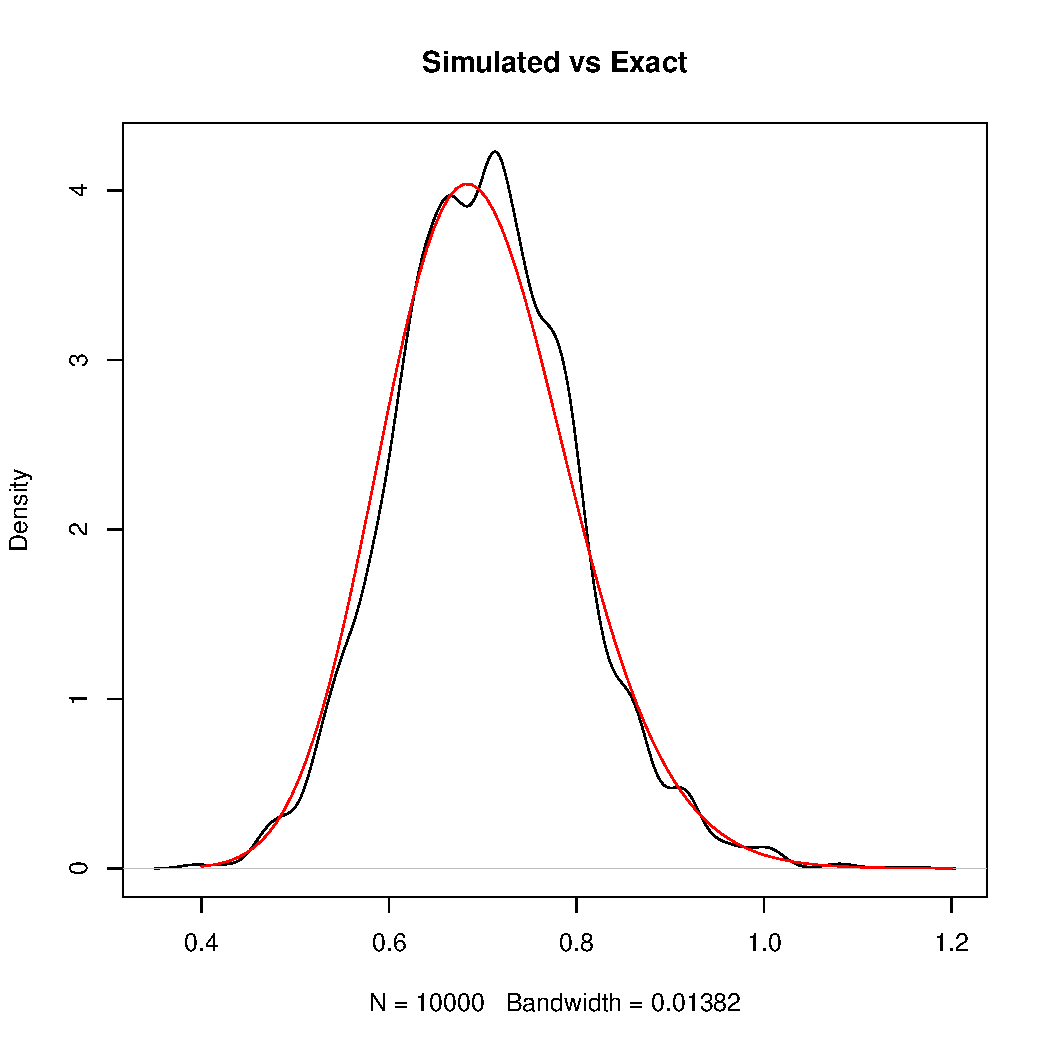
\includegraphics[width=0.60\linewidth]{figure/unnamed-chunk-4-1} 

\end{knitrout}
\section*{Exercise 4}
Let $R \sim exp(1)$, $M \sim exp(\frac{1}{2})$, $S \sim exp(\frac{1}{3})$. Also note that 25 minutes is $\frac{5}{12}$ hours. 
\begin{equation}
\begin{split}
p(min(R,M,S)>25*1/60) = 1-exp(-(1^{-1}+(1/2)^{-1}+(1/3)^{-1})*5/12)=1-0.082085
\end{split}
\end{equation}
\section*{Exercise 5}
Let $p=\frac{1}{50}$, $n=20$
$binom(20, 1/50)$,so $\frac{\lambda}{n}=\frac{\lambda}{20}=1/50 \implies \lambda = 2/5$ and $\therefore binom(20, 1/50) \approx Poisson(2/5)$
\begin{equation}
p(k\geq 1) = 1 - p(k=0) = 0.32968
\end{equation}
\section*{Exercise 6}
$T_1$ be the expected value of the amount of time that the first navigation lasts. There are three possible senarios when that can happen, \{1 or 2 dies before t and 3 dies at t\}, \{1 or 3 dies before t and 2 dies at t\}, \{2 or 3 dies at t and 1 dies at t\}
\begin{equation}
\begin{split}
f(time) = (p(T_1 >t)p(T_2 \leq t)+p(T_1 \leq t)p(T_2>t))*p(T_3=t) + \\
(p(T_1 >t)p(T_3 \leq t)+p(T_1 \leq t)p(T_3>t))*p(T_2=t) + \\
(p(T_2 >t)p(T_3 \leq t)+p(T_2 \leq t)p(T_3>t))*p(T_1=t) = \\
(exp(-t)*(1-exp(-2/3t))+(1-exp(-t))*(exp(-2/3t)))*1/3*exp(-1/3t)+\\
(exp(-t)*(1-exp(-1/3t))+(1-exp(-t))*(exp(-1/3t)))*2/3*exp(-2/3t)+\\
(exp(-2/3t)*(1-exp(-1/3t))+(1-exp(-2/3t))*(exp(-1/3t)))*1*exp(-t)=\\
4/3exp(-4/3t)-4/3exp(-2t)+exp(-t)-exp(-2t)+5/3exp(-5/3t)-5/3exp(-2t)=\\
4/3exp(-4/3t)+exp(-t)+5/3exp(-5/3t)-4exp(-2t)
\end{split}
\end{equation}
\begin{equation}
\begin{split}
E(t) = \int_{0}^{\infty} t*(4/3exp(-4/3t)+exp(-t)+5/3exp(-5/3t)-4exp(-2t)) dt = \\
4/3\int_{0}^{\infty} t*(exp(-4/3t)) dt + \int_{0}^{\infty} t*(exp(-t)) dt + \\ 5/3\int_{0}^{\infty} t*(exp(-5/3t)) dt - 4\int_{0}^{\infty} t*(exp(-2t)) dt = \\
3/4+1+3/5-1 = 1.35
\end{split}
\end{equation}


\end{document}
